\section{Datenverarbeitung}
	
	In diesem Kapitel wird näher auf den Programmcode des vorliegenden Forschungsprojektes eingegangen und erklärt was genau wir in der Datensammlung und 
	Datenverarbeitung gemacht wurde. 
	Als erstes haben wir die Daten wie in Punkt 2.1.1 beschrieben mit der Bibliothek gescrapped und als csv-Datei abgespeichert. Wie das Sracpping in der 
	Bibliothek genau funktioniert ist ebenfalls unter dem Punkt 2.1.1. GetOldTweets beschrieben. Um die gespeicherten Tweets für das Mapreduce vor zu 
	verarbeiten nutzen wir die zur Verfügung stehenden Bibliotheken NLTK und cleantext.
	
	
	\begin{figure}[ht]
		\centering
		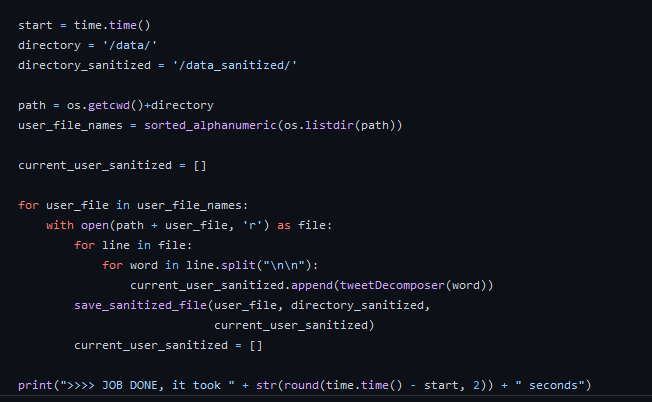
\includegraphics[width=0.9\textwidth]{images/Kapitel2/Code_Datensanierung_1}
		\caption{\label{fig:DataSan}Sanierungs-For-Schleife der Daten}
	\end{figure}
	
	Die Variable "directory" und "directory\_ Sanitized" geben den Path an, in welchen Ordner die Daten gespeichert werden sollen. mit der bibliothek os von Python 
	kann man zum Beispiel über "os.listdir(Path)" alle Dateinamen innerhalb dieses Ordners einlesen lassen. 
	Über die Variable user\_ file\_ names bekommen wir eine Alphanumerisch sortierte Liste der Usernamen der Politiker zurück, welche wir dann über eine For-
	Schleife durchgehen, da der Name der CSV-Dateien folgenden Muster entspricht, "Name\_ D" oder "Name\_ R". D steht für demokratisch und R für 
	republikanisch. In dieser Datensanierungsschleife wird die Funktion tweetDecomposer verwendet. Diese Funktion übernimmt in der vorliegenden Datensanierung die 
	Hauptaufgabe.\\
	
%	\begin{figure}[ht]
%		\centering
%		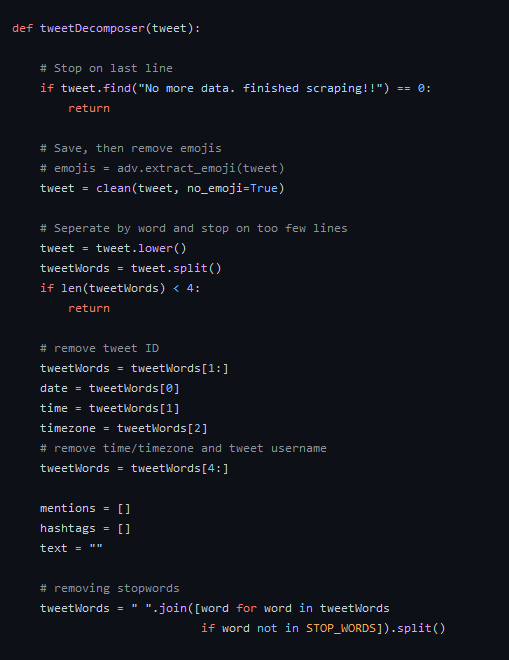
\includegraphics[width=0.9\textwidth]{images/Kapitel2/Code_Datensanierung_2}
%		\caption{\label{fig:DataSanF1}Ausschnitt eins der Sanierungsfunktion der Daten}
%	\end{figure}

	Mit dem Bibliothek cleantext wurden die emojis aus dem Text entfernt, wie man in Abbildung ~\ref{fig:DataSanF1} in den ersten Zeilen der Funktion sehen kann.
	Dann werden alle Worte innerhalb eines Tweets klein geschrieben und aufgetrennt, damit dann  die ID, die Zeitzone und der Username aus dem Tweet entfernt 
	werden kann. Mit NLTK werden dann die Stoppworte durch ein join aus den Tweets entfernt, so das man zu den letzten Datensanierungsschritten kommen kann.\\
	 
%	\begin{figure}[ht]
%		\centering
%		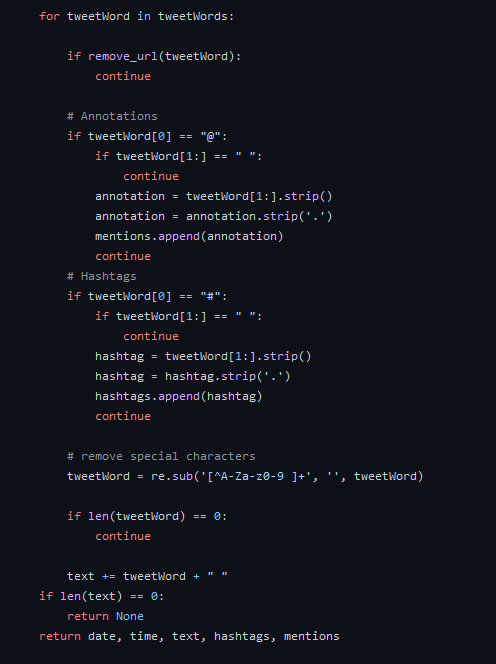
\includegraphics[width=0.9\textwidth]{images/Kapitel2/Code_Datensanierung_3}
%		\caption{\label{fig:DataSanF1}Ausschnitt eins der Sanierungsfunktion der Daten}
%	\end{figure}
	
	Da die Annotations und Hashtags gespeichert werden sollen, wurde, wie in Abbildung ~\ref{fig:DataSanF2} zu sehen, ist eine extra For-Schleife. Die for-Schleife läuft über 
	den gesamten Input des Tweets, dazu zählt Datum, Zeit, Username, Hashtags,Emoji usw. Als erstes wird überprüft ob es sich um eine URL handelt oder nicht. Tritt der Fall 
	ein das es eine URL ist wird diese einfach übersprungen und nicht mit abgespeichert. Die Annotations können durch eine "@" erkannt werden, während die Hashtags mit 
	einem "\# " erkannt werden. Beide Erkennungsmaker werden nicht mit abgespeichert. Der restliche Inhalt des Hastags und der Annotation werden in einer Liste gespeichert. 
	Als letztes haben wir alles Spezielle Charakter, wie Punkte, Kommas, usw. entfernt aus den tweetword. Die Funktion gibt dann alle interessanten Daten für die Analyse 
	zurück.Zum Schluss werden diese Daten in einer CSV-Datei gespeichert Ordner data\_ sanitized.  
	Als nächster Schritt folgt die Hauptanalyse unseres Projektes in 2.3. 
	
	
